% ============================
%          ABSTRACT/INTRODUCTION
% ============================

\chapter*{Introduction\markboth{Introduction}{}} 
\addcontentsline{toc}{chapter}{Introduction}
This thesis describes the development and applications of a laser turret with pan and tilt control: this device can be used to project a laser dot on a given surface (wall and/or floor) and finely control its position by solving the system’s inverse kinematics.

Once its functionality was validated, we used the turret for a human-robot interaction task.  In particular, we considered an existing system in which an operator interacts with a drone using pointing gestures \cite{gromov2018robot}; the system initially determines the relative localization between the two, then allows the operator to control the drone, which follows the indicated location in real time. The existing approach relied on a fast agile robot, and was unsuitable for implementation on slower or larger ground robots.  In this thesis, we demonstrate how the turret can be used with this goal. Figure \ref{fig:preview} gives an idea.
\begin{figure}
	\centering
	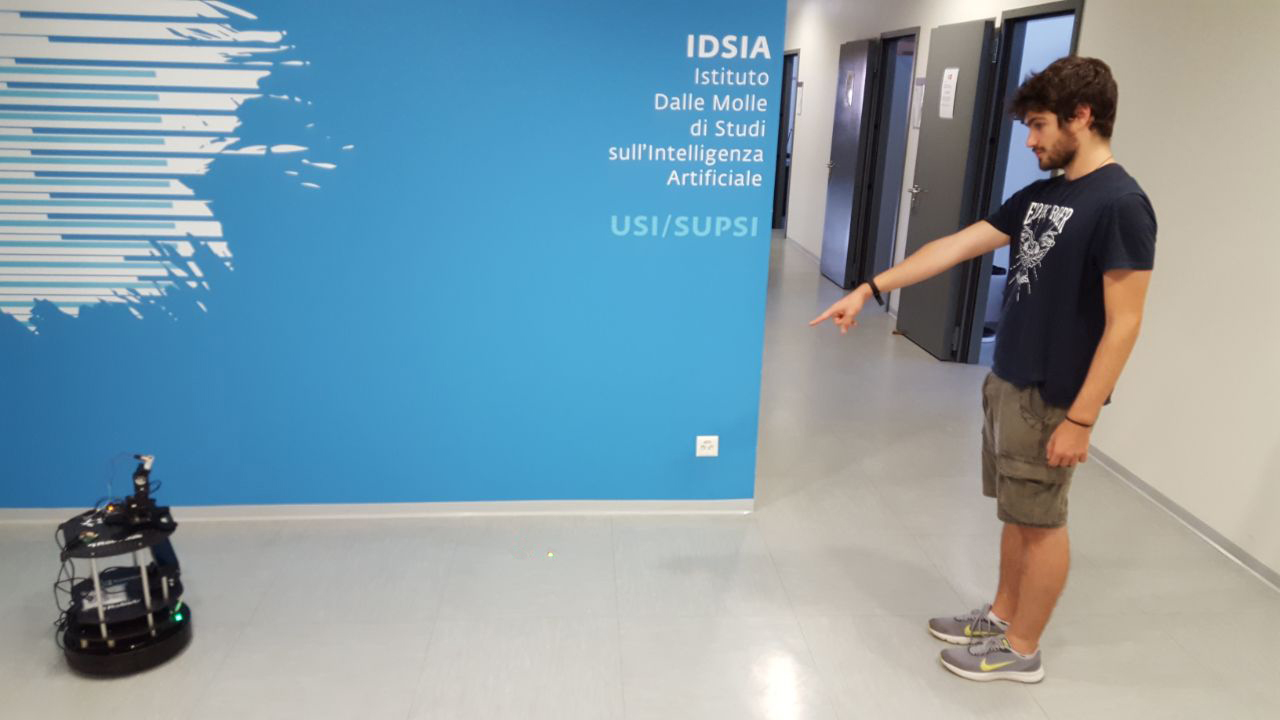
\includegraphics[width=\textwidth]{img/preview.jpg}%
	\caption{System Deployed to Drive a Ground Robot}
	\label{fig:preview}
\end{figure}

Finally, the turret was adopted to efficiently run experiments for fine tuning or validating different components of the system described above, such as the algorithms for relative localization and the algorithms for reconstruction of the pointed direction.  To this end, we ran an experimental campaign involving ten users.

\section*{Motivations and Related Works} \label{sec:related}
Many works in the field of \ac{HRI} involve the study of interactions between an operator deployed alongside a robot in an environment they share. That means that a direct line of sight exists between the two. Many interfaces have been proposed, ranging from standard joysticks to hands-free gesture-based interfaces based on sensorized armbands~\cite{Wolf2013}, bracelets~\cite{Cacace2016,gromov2018video}, smartwatches~\cite{Villani2017} or voice commands~\cite{Gromov2016}.

The system developed in this thesis is collocated in that context, thus, an overview of related works is useful to understand motivations that stand behind that project.

\subsubsection*{Pointing Based HRI Interface}
\emph{Pointing gestures} can be a solid possibility for proximity interaction techniques.
As a matter of fact, they can be used to intuitively express locations or objects with minimal cognitive overhead; there are many examples in \ac{HRI} research, and we are going to recall them in the next section.

First, a differentiation can be made on sensing with respect to the type of sensors involved and their locations with respect to the human: it can be either \emph{external} or based on \emph{wearable} devices.
External sensing is commonly built upon vision systems, like stereo cameras \cite{Nickel2003}, \acs{RGB} cameras \cite{Pateraki2014,Monajjemi2016},  structured light depth cameras \cite{Cosgun2015} and \ac{ToF} cameras \cite{Droeschel2011}. The wearable sensing is usually realized either with inertial \cite{Wolf2013,Sugiyama2013} or magnetic measurements \cite{Bolt1980,Nickel2003}. 

Our work is an example of wearable sensing, as we exploit a wearable \ac{IMU} device. We are interested in such type of sensing because, even if vision-based offers some advantages, being able to obtain useful information about objects, like speed, shape, colour and size, they have also some major drawbacks, like being influenced by poor lighting conditions, low spatial resolution and, last but not least, being in need for high computational resources.
Thus, for proximity interaction, wearable sensing is a very interesting possibility.

In particular, the use of pointing gestures constitutes a very practical and profitable solution, being based on mechanics which are natural for humans. This explain the amount of effort made so far into that research topic, which has produced many pointing gestures solutions in \ac{HRI} field.

In fact, we have acknowledgment of pointing gestures being used as an input interface already in 1980, with the work presented by Bolt, \virgolette{Put-that-there}~\cite{Bolt1980}. Moreover, pointing gestures are often used for system which need to select a robot within a group~\cite{Nagi2014a,Pourmehr2013}, pick-and-place tasks~\cite{Brooks2006,Droeschel2011,Grossmann2014,Cosgun2015}, labeling and/or querying information about objects or locations~\cite{Brooks2006,Pateraki2014,Akkil2016}, and providing navigational goals~\cite{VanDenBergh2011,Abidi2013,Wolf2013,Jevtic2015,Gromov2016,Tolgyessy2017}.

Providing navigational goals is exactly the field in which our system finds one of its main applications and this is why we are now going to mention more works related to that task. First, however, it is worth to say that one important issue to be solved in natural human-robot interaction that involves pointing is a perception of the user's gestures. That responsibility can be left directly to a robot, as well as of a group of cooperatively-sensing robots~\cite{Giusti2012,Pourmehr2013}; of the environment~\cite{zivkovic2008toward}; or, as in our case, of a device worn by the user~\cite{Sugiyama2013,Wolf2013,Gromov2016}. The first approach is the most popular in \ac{HRI} research. However, it presents important challenges to solve the perception problem, and requires the robot to consistently monitor the user. Relying on sensors placed in the environment relaxes the requirements on the robots, but limits the applicability of the system to properly instrumented areas; in both cases, the positions being pointed at need to be inferred by external observation, which is typically performed with cameras or \acs{RGB-D} sensors.

\subsubsection*{Providing Navigational Goals}
Van Den Bergh et al. \cite{VanDenBergh2011} used pointed directions to help a ground robot to explore its environment. The robot keeps looking for a human in its area and once detected starts the interaction. Using an \acs{RGB-D} sensor (Microsoft Kinect) the system detects human's hand and wrist. A vector connecting the center of the hand and the wrist is then projected on the ground, providing an exploration direction. Finally, the next exploration goal is automatically obtained from a set of possible goals with respect to an instantaneous occupancy grid acquired by the robot. 

Similarly, Abidi et al. \cite{Abidi2013} use a Kinect to extract pointed directions. Navigation goals are continuously sent to the ground robot, which immediately plans its motion and thus allows the user to rapidly correct his input. The main drawback, however, is that the robot has to keep looking at the user in order to reach the final destination. To reconstruct human pointing authors suggest two approaches: the first is a vector with origin in the elbow and passing through the hand/finger, the second is the same vector, but originating from the eyes.

Jevtic at al. \cite{Jevtic2015} experimentally compared different interaction possibilities in a user study involving 24 people. A ground robot equipped with a Kinect and other sensors was used. The study compares three interaction modes: \ac{DPI}, person following, and pointing control in area- and waypoint-guidance tasks. The DPI mode requires the user to push the robot by hands, the torques generated at motors are measured via electrical current and then are fed to a friction-compensation controller that drives the robot in the appropriate direction. The person following mode consist in the robot following the user at a safe distance; the user can stop the robot in any moment by raising his left hand above the left elbow and thus be able to control the robot's precise location. The pointing mode allows the user to command the robot's position with a pointing gesture, where the target location is calculated from the intersection of the ground plane with a line passing through the right elbow and the right hand of the user.
The authors measured task completion times, accuracy, and workload (with NASA-TLX questionnaire). Results show that the DPI mode is systematically better than the other mode for all metrics, while the pointing control shows the worst results.

Those bad performances of the pointing interface can be explained with the absence of a proper feedback and a time-sparse nature of the implemented gesture control: the user issues only one command to drive the robot to a goal and see how the system has interpreted his pointing only when the robot reaches the target. In that way, the user cannot correct the robot's position properly. This problem is nicely solved by our system, as it provides a real-time feedback to user pointing with a laser pointer, making him able to understand where the system thinks he is pointing and also correct any misalignment.

Moreover, also the pointing model proposed (elbow-hand) is proved to be intrinsically imprecise. As a matter of fact, many other studies, including those from the psychology research, demonstrate that a proper model would consist of a vector that passes through the head and the fingertip (\cite{Taylor1988,Herbort2016,Abidi2013,Nickel2007,Droeschel2011}. 

\subsubsection*{Wearable Sensors}
An alternative approach for the perception of pointing gestures is wearable sensors, as we mentioned before. 

Sugiyama et al. \cite{Sugiyama2013} developed a wearable visuo inertial interface for on site robot teaching based on a combination of \ac{IMU} and monocular camera  to capture hand gestures from the user point of view. The camera is also used for a monocular \ac{SLAM}, which allows to localize the user with respect to the robot coordinate frame.

Wolf et al. \cite{Wolf2013} propose a gesture-based interface for a robot control, that is based on a device called BioSleeve, a wearable device located on the user's forearm and comprised of a set of dry-contact surface \ac{EMGs} and an \ac{IMU}. Optionally, the authors suggest to strap an additional \ac{IMU} sensor on the upper arm to be able to perform a model-based arm pose reconstruction for pointing gestures. However, no information is provided on how a user would localize herself with respect to the robot in order to control its position.

A work by Villani et al. \cite{Villani2017} suggests to use a single smartwatch device to control a drone. The system provides two interfaces: high-level commands and velocity commands.

Cacace et al. \cite{Cacace2016} demonstrate a multi-modal human-robot interface used for interaction in search and rescue missions. The operator is equipped with a Myo armband used for gestures, headset for voice commands, and a tablet with a touch screen.

\section*{Document Structure}
The rest of the document is structured in chapter as follows:
\begin{itemize}
    \item \textbf{Chapter 1 - Models Specification}  All the geometric models and formulas on which the system is based are explained. This includes turret model, human pointing model and relative localization procedure;
    \item \textbf{Chapter 2 - Hardware Implementation}  We introduce all the hardware components involved in the development of the presented system: servo motors and interface board for the turret, arm IMU devices and the ground robot used for demonstrations;
    \item \textbf{Chapter 3 - Software Implementation} We give an overview of the main libraries used and then describe the entire project software implementation;
    \item \textbf{Chapter 4 - Experiments and Applications} We describe the experiments the turret system allowed us to perform and show possible application scenarios developed;
    \item \textbf{Chapter 5 - Conclusion and Future Work} We make a brief recap of the thesis, draw some conclusions and report eventual further improvements or possible works;
    \item \textbf{Appendix A} Here we collect a couple of things that did not find a place in the main document, but can be interesting to mention;
    \item \textbf{Appendix B - Code Listing} Relevant code listings.
\end{itemize}
